\chapter{India is a Geographical Entity}

March 24, 2016
\vskip 2pt

Dear Members of the Instructional Quality Commission and the California Board of Education:
\vskip 2pt

Greetings!
\vskip 2pt

I am writing to contest some of the edits as suggested by South Asia scholars, and appeal to your good offices to consider and weigh the truth of our contestations. These edits primarily concern the replacement of India with South Asia. Given that the revisions suggested are for History and Social Sciences, it is extremely important that we do not replace India with South Asia. The geo-political category of South Asia is a relatively new construct whereas India has a long history of geographical and civilizational existence and representation. As long as one can go back in recorded history, one finds the mention and representation of India as a civilization and culture. As a geographical and civilizational unit, India has been on the forefront of inter-cultural, economic, and military interaction with the rest of the world. Replacement of India with South Asia tantamounts to erasing the history of our shared humankind. India since antiquity has interacted with the people from Greece, Rome, Persia, Arabia, Ethiopia, China, Japan, Korea, Java, Sumatra, Bali, Cambodia, England, France, Spain, Portugal, Germany, Italy, the United States, and so many other empires, regions, or nations of the past and the present. It becomes especially pertinent that when we do not erase the names of ancient civilizations like Greece, Egypt, and China that we do not do away with India either.

In our western conceptualization, the idea of India as one unit is as old as the early Greeks. Herodotus (484--425 BCE), the Greek historiographer, mentions India and Indians in the context of Darius I and his conquests. India is represented as one of the twenty satrapies of Darius’s Empire, paying maximum treaty—360 talents of gold per annum. The Persian army also had an Indian contingent and they were mentioned as such:\footnote{This letter and the following one in the appendices, was originally written with APA style for references and citations. Whereas we have used the Chicago Manual for the book, we have left the APA format of the letters unchanged.}
\begin{quote}
The Indians wore garments made of cotton and carried bows and arrows of reed. In addition they had iron weapons. [Cited in Parker, 2011, p.\ 24]
\end{quote}
Herodotus also mentions of Indians living far in the South as people not under the rule of the Achaemenid Empire—this basically suggests that there was a section of India and Indians who were under the rule of Darius I and there were others, who were outside his pale.

The description of India as a unit by Herodotus is preceded by Hecataeus of Miletus, who is known to have created a map in the shape of a disc of the world as known to the Greeks then. The river Indus and India were on the easternmost fringes. This was further preceded by Scylax’s \textit{Indica}, which contained descriptions of and on India. Darius I was supposed to have employed Scylax to survey the river Indus, an enterprise which helped him to bring parts of India under the Achaemenid Empire.

Megasthenes’ \textit{Indica}, written anytime between fourth century and third century BCE, provides further credibility to India’s existence as he emphasizes in its territory what is considered its eastern part currently, for he describes a city which is modern day Patna, the capital of Bihar—one of the eastern states of India. He calls it a land of exceptional beauty and abundance, resourced with gold, silver, iron, copper, gems and objects of all kinds that constitute wealth and luxury. He was in all probability a Greek ambassador in the court of Chandragupta Maurya, king Ashoka’s grandfather. 

Eratosthenes (276--196 BCE), the polymath librarian of Alexandria who was also a geographer known to have calculated the circumference of the earth and for constructing a map on latitudes and meridians saw India as one unit, for he writes: “If the enormity of the Atlantic ocean did not prevent it, we would be able to sail from Iberia to India along the same parallel over the remainder of the circle” [cited in Parker, 2011, p. 53]. Since the ancient times, the river Indus has been a defining feature in the consciousness of the foreigners dealing with India in their writings, travels, or invasions. Eratosthenes, using stade as a unit of measurement, contended that the distance between the river Indus and eastern India was 16000 stades. This clearly shows once again that it was not India around Indus which was in consideration of the Greeks; it was the entire subcontinent around Indus as well as to the east of Indus. Parker (2011) writes that Eratosthenes represented India on his map in the form of a diamond shaped quadrilateral in a manner more distinct as any other country or geographical unit. His descriptions were later picked up by Strabo and Ptolemy. 

The idea of India as one geographical unit is also present in the writings of Arrian in \textit{Indica}. Arrian wrote this work based on the writings of Megasthenes and Nearchus, who was an admiral in the fleet of Alexander, which was prepared during his return to sail through the river Jhelum and Indus to the Persian Gulf. He also included in the earlier portions of the work the geographical contentions of Eratosthenes. Parker (2011) writes: 
\begin{quote}
Arrian devotes the second and third chapters of his \textit{Indica} to describing the geographical shape of India, as if on a diagrammatic map. He is careful to define it in terms of its borders: to its west is the Indus, to its north Mount Taurus or Caucasus, to its south the Great Sea; about the east there is no clarity. (p.\ 87) 
\end{quote}
There was no clarity for Arrian regarding the east because Alexander had not gone past Hyphasis: “But I can make no accurate assertion about territory on the other side of the Hyphasis, because Alexander did not go beyond Hyphasis” [Cited in Parker, 2011, p. 38]. 

Strabo’s (64/63 BCE—21 CE) \textit{Geography} is another seminal text from the ancient times, which gives an extensive coverage to India. He divides the world into four parts, and one of them was India. In the seventeen books authored by Strabo, India makes two major appearances in them (Parker, 2011).

\centerline{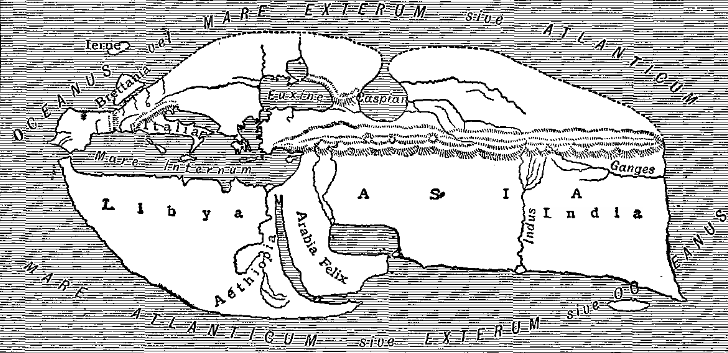
\includegraphics{figures/appendix-a-fig1.png}}

India finds mention in Ptolemy’s (90--68 CE) \textit{Geography} as well—in the seventh book. Both the rivers Indus and Ganga find mention. The Indian peninsula is included as well, though shortened. It is compensated by a larger depiction of present day Sri Lanka.

Pliny, the Elder (23/24--79 CE) continues with the theme of discussing India as a distinct and separate unit. His \textit{Natural History} has a separate section of India, following which he discusses Sri Lanka (\textit{Taprobane}). \textit{When we take into account, the accounts of both Ptolemy and Pliny, the exclusive emphasis on India distinct from present day Sri Lanka makes it clear that they we were not talking about present day South Asia in reference to India, for Sri Lanka today is part of South Asia but it was not part of India when India was being discussed historically.} 

Given that India is spoken about, there is mention of Indians as well. The different commentators have spoken about the characteristics of the Indian people. Strabo states that India had encountered two invasions before Alexander but they were both repulsed. The Indian people, according to him, were unwarlike; however they were well-behaved during the war (this is understandable given the social codes pertaining to war as mentioned in texts on the social behavior of the Indians). Diodorus mentions that during wars, there was a custom to leave the agricultural workers undisturbed—this also is in tune with the social rules governing the Indian people in the traditional texts involving the governance of social behavior. Diodorus also states that despite the division of the society in different categories there was no prevalence of slavery, as fundamental freedom was guaranteed to all and sundry. Given the exclusive emphasis of inequality of the ancient Indian society in the letters of South Asia scholars, it may be worthwhile to look at the complete quote from Diodorus: 
\begin{quote}
Concerning the customs of the Indians which are unique to them, one may consider that which was drawn up by their ancient sages to be the most remarkable, for it has been decreed that under no circumstances shall anyone among them be a slave, but that everyone shall be free and honor the equal status of all persons. [Cited in Parker, 2011, p.\ 89]
\end{quote}
Drawing on Megasthenes, Strabo describes the ancient Indian people as simple and honest—not given to crowd behavior, drinking other than on special occasions, theft, or litigations.

The above examples get amplified and multiplied if we take into account the Persian, Turkish and Chinese accounts for India and Indians. Chinese travellers Fa-hien (4th century CE) and Xuanzang (7th Century CE) describe the country that they visited as \textit{Shintu} or Hindu/India and their description leaves no one in doubt that they are referring to various parts of the Indian subcontinent as belonging to one civilization. Similarly the Arabs and Persians called India as Hind and Indians as Hindus. 

As far as the Indians themselves are concerned, they called the entire subcontinent Bharat and Jambudwipa. One of the earliest mentions of India as one unit comes from one of the four Vedas—the \textit{Atharvaveda}. It likens the Indian subcontinent as a tortoise, and describes its each and every part. \textit{Vishnu Purana} (500 CE or earlier) clearly defines the borders of India as the land between the Himadri Mountains and the ocean. Other \textit{Puranas} mention the subcontinent as Bharatkhanda and Bharatvarsha. 

I can quote numerous sources in each category to substantiate our point; however I am limiting myself to primarily the Greek as well as the Roman sources given their familiarity to most of you. The idea primarily is that given the historicity of India as a geographical and civilizational unit and given its place in world history as one of the major civilizations of the world since antiquity, I would request you to not replace India with South Asia. Yes, there are places where the Indian subcontinent could be used, and I support the replacement. \textit{The edits that have been submitted by Uberoi Foundation have my backing}.

\begin{thebibliography}{99}
\bibitem{apx-a-key1} Parker, P. (2011). \textit{The making of Roman India}. Cambridge, MA: Cambridge University Press.
\end{thebibliography}
